\chapter{Simulation Procedure}
\label{chp:MAT}
%%%%%%%%%%%%%%%%%%%%%%%%%%%%%%%%%%%%%%%%%%%%%%%%%%%%%%%%%%%%%%%%%%%%%%%
A simulation study was conducted which allows changing parameters of interest (i.e. the number of target statistics and number of simulations). All simulations and analyses were conducted using R version 3.6.2 (2019-12-12)

\section{Simulation Setup}


\begin{table}[h!]
\begin{center}
	\caption{Simulation Setup for Calibration Methods}
	\begin{tabular}{ |c|c|c| } 
		\hline
		 & Scenario One & Scenario Two \\
		 \hline
			\multirow{2}{*}{Targets features} & Prevalence at times 50 and 75 & Prevalence at times 50 and 75 \\
			& &+ peak prevalence \\ 
		\hline
		
	\multirow{3}{*}{Targets used}	 & Prev. at 50 = 0.644 (644 out of 1000)
		
		 & Prev. at 50 = 0.622 (622 out of 1000)\\
		 
		 &	Prev. at 75 = 0.404 (404 out of 1000) &
		 Prev. at 75 = 0.371 (371 out of 1000)\\
		 
    	&	& Peak prev. = 0.677 (677 out of 1000)\\
		  
		\hline
		
		Number of\\ simulations & 60,000 & 75,000 \\
		\hline
		\multirow{3}{*} Parameters & Beta = 0.2 & Beta = 0.2 \\
    	used to & Gamma = 0.02 & Gamma = 0.02 \\
	generate targets & &\\
	\hline
		\multirow{3}{*} Initial & S=990 & S=990 \\
		compartmental & I=10 & I=10 \\
		values & R=0 & R=0 \\
		\hline
	\multirow{2}{*}{Time span} & Sequence from 0 to75 &Sequence from 0 to75\\
	& incremented by 1 & incremented by 1\\
		\hline
		Beta prior & Uniform distribution (0,1) & Uniform distribution (0,1)\\
		\hline	
		Gamma prior & Uniform distribution (0,0.5) & Uniform distribution (0,0.5)\\
		\hline
		
	\end{tabular}
\end{center}
\end{table}


\begin{table}[h!]
	\begin{center}
		\caption{Simulation Setup for the Reference}
		\begin{tabular}{ |c|c|c| } 
			\hline
			& Scenario One & Scenario Two \\
			\hline
			\multirow{2}{*}{Targets features} & Prevalence at times 50 and 75 & Prevalence at times 50 and 75 \\
			& &+ peak prevalence \\ 
			\hline
			
			\multirow{3}{*}{Targets used}	 & Prev. at 50 = 0.644 (644 out of 1000)
			
			& Prev. at 50 = 0.622 (622 out of 1000)\\
			
			&	Prev. at 75 = 0.404 (404 out of 1000) &
			Prev. at 75 = 0.371 (371 out of 1000)\\
			
			&	& Peak prev. = 0.677 (677 out of 1000)\\
			
			\hline
			
			Number of\\ simulations & 1,000,000 & 1,000,000 \\
			\hline
			\multirow{3}{*} Parameters & Beta = 0.2 & Beta = 0.2 \\
			used to & Gamma = 0.02 & Gamma = 0.02 \\
			generate targets & &\\
			\hline
			Beta prior & Uniform distribution (0.1,0.4) & Uniform distribution (0.1,0.4)\\
			\hline	
			Gamma prior & Uniform distribution (0.01,0.03) & Uniform distribution (0.01,0.03)\\
			\hline
			
		\end{tabular}
	\end{center}
\end{table}

\section{Obtaining Targtes}
As target statistics in this study, there were two scenarios. Scenario one (S1) considered two target features (prevalence at two-time points, 50 and 75) and scenario two (S2) looked at three target features (peak prevalence for each model run in addition to the two-time points in scenario one).


\begin{figure}[h!]
	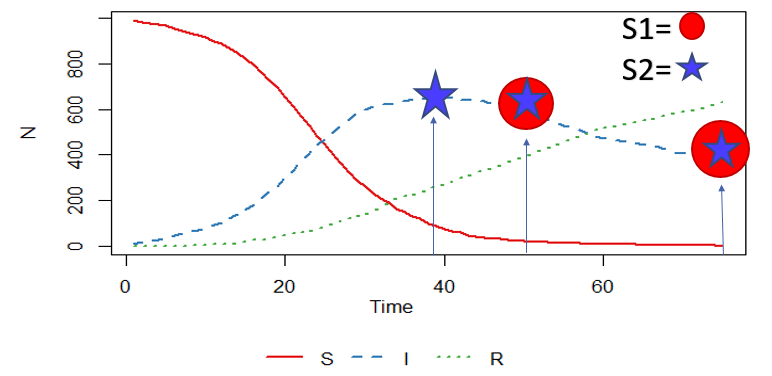
\includegraphics[width=\linewidth]{targets.png}
	\caption{targets for scenarios 1 and 2. Scenario 1 considers only green points on the     Infectious (I) curve while scenario 2 considers both red and green points on the (I) curve}
	\label{targets}
\end{figure}

R version 3.6.2 (2019-12-12) was used to perform the statistical analyses and datasets were obtained from a stochastic SIR model using the SIR function in the SimInf library \cite{siminf}. To obtain targets for scenario one, the SIR model was ran once with known parameter values $\beta = 0.2, \gamma = 0.02$ and the prevalence at times $50$ and $75$ were saved as target statistics. Similarly for scenario two, the SIR model was ran once with the same known parameter values and the prevalence at times $50$ and $75$, as well as the peak prevalence, were saved as targets (see Figure \ref{targs1,targs2} below).


\begin{figure}[h!]
	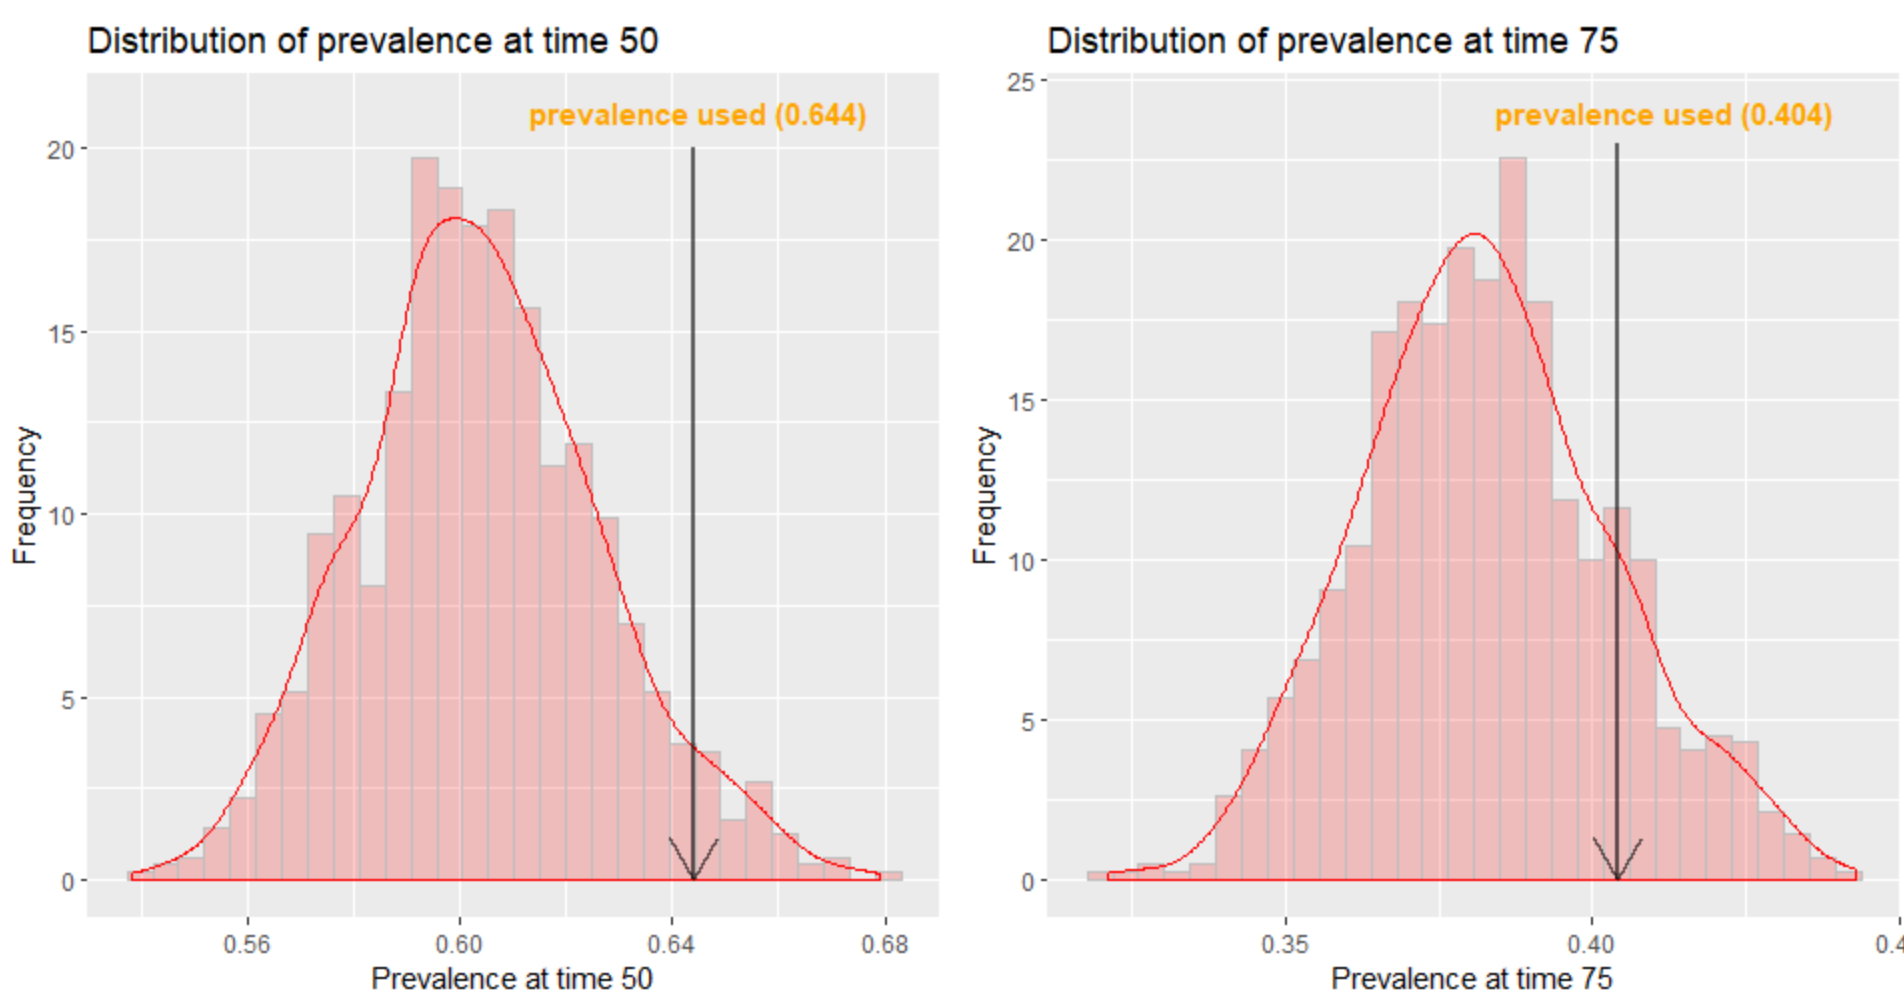
\includegraphics[width=\linewidth]{targ_dist_S1.png}
	\caption{Distribution of targets in Scenario 1 }
	\label{targs1}
\end{figure}


\begin{figure}[h!]
	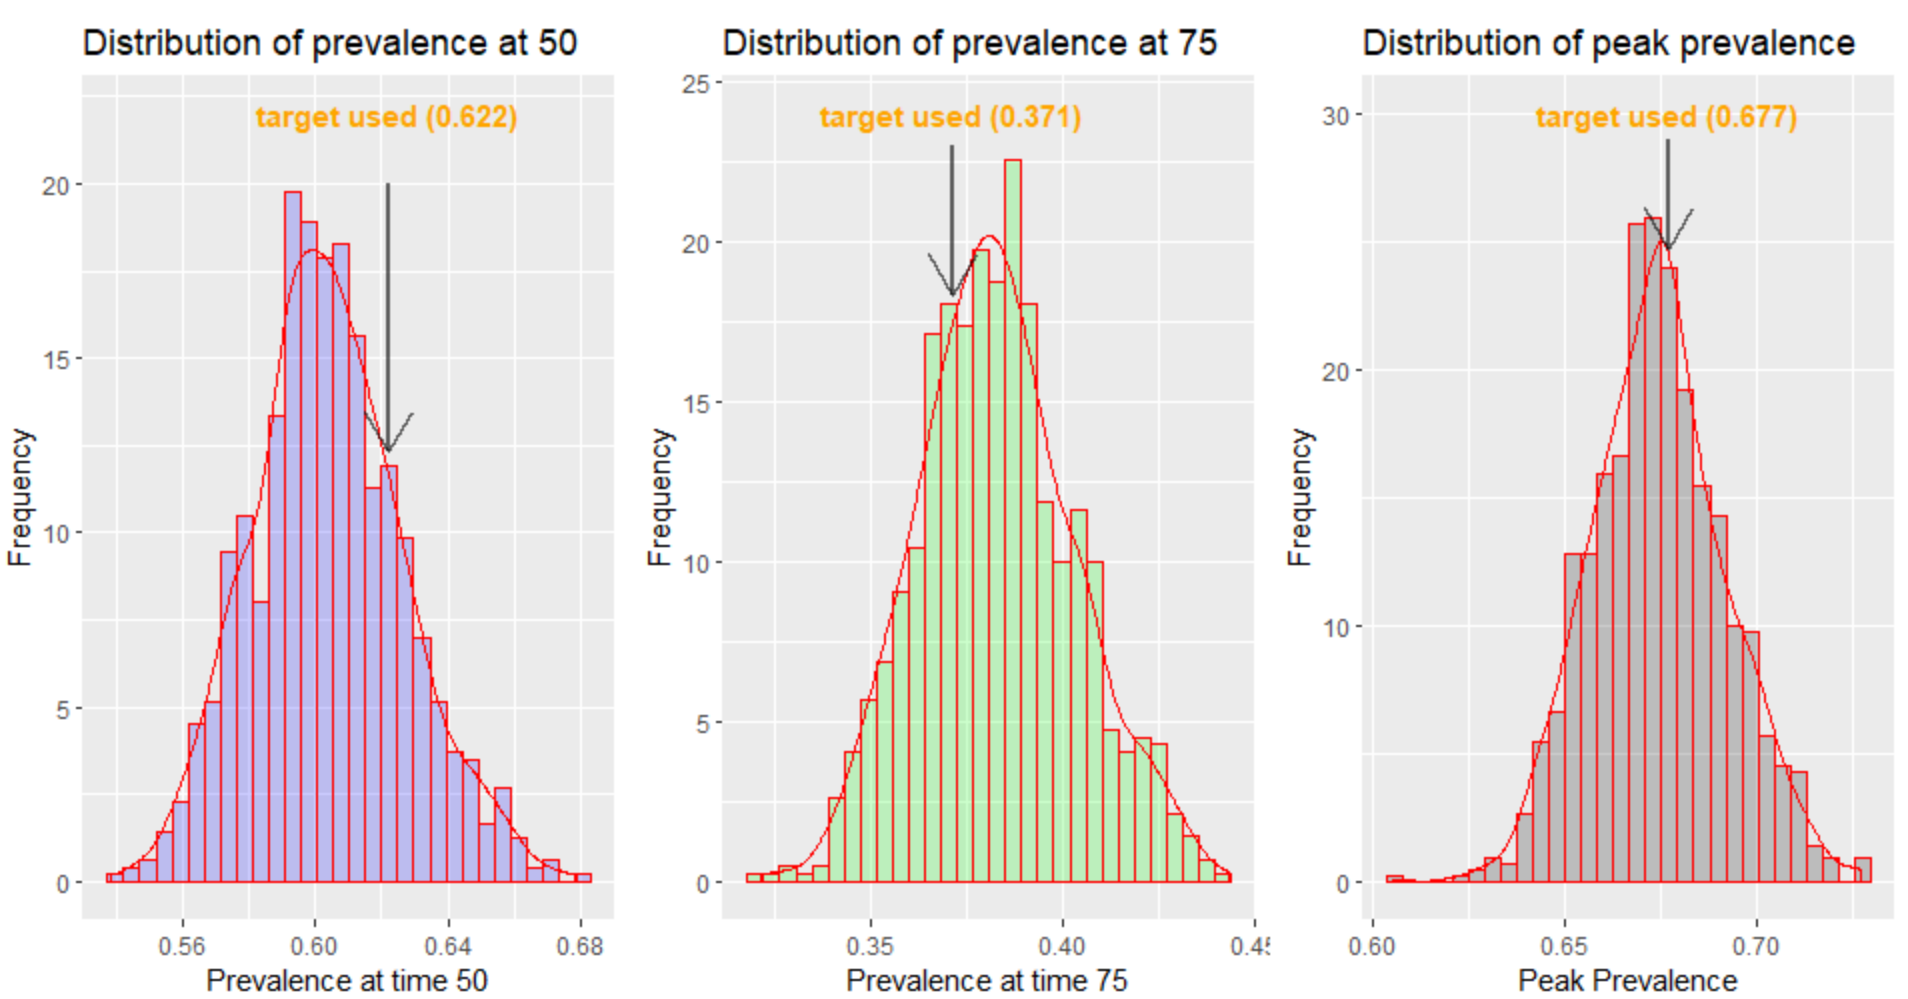
\includegraphics[width=\linewidth]{targ_dist_S2.png}
	\caption{Distribution of targets in Scenario 2 }
	\label{targs2}
\end{figure}
